\clearpage
\chapter{Form Basics}

\classquote{夫人之立言，因字而生句，积句而成章，积章而成篇。\\
When people set words down, characters give rise to sentences, sentences gather into sections, and sections gather into a whole piece.}{The Literary Mind and the Carving of Dragons · Chapters and Sentences}{Characters make sentences, sentences make sections, sections make a whole—the same ladder as motive, phrase, section, piece. Form is not a template to fill in; it is a plan for what the listener should remember, expect, and finally receive.}

\label{sec:form-basics}

\section*{What you can do after this chapter}
\begin{itemize}
  \item Break a song into functional sections instead of describing it only as ``a few continuous passages.''
  \item Organise four-bar phrases into eight-bar, sixteen-bar, or full-song structures with repetition, variation, and contrast.
  \item Recognise AABA and verse--chorus forms, and explain the strengths and risks of each.
  \item Design a transition that actually lands, then lay the structure out in Yeban's arrangement view with clip copy, paste, and the section band.
\end{itemize}

\section{Form: dividing time into memorable levels}

Form is the organisation of a piece over time. It does not answer ``is this passage good?'' It answers ``what is each passage responsible for, and why does the next one start here?'' The same chord loop repeated three times as an eight-bar section sounds different from the same material arranged as verse--chorus--verse--chorus. The material did not change; its position and function did.

Form has levels. The smallest unit is the motive, usually one or two bars. Several motives make a phrase, often four or eight bars. Several phrases make a section, often eight to thirty-two bars. Several sections make the whole song. The previous chapter grew a motive into a phrase; this chapter puts phrases into sections and sections into a song.

The levels are not defined by bar counts alone. An eight-bar section may contain one long phrase; a four-bar section may contain two two-bar phrases side by side. To identify a section, first ask whether it has its own opening, development, and close, then ask whether it does a different job from its neighbours. Names such as verse, chorus, and bridge are functional names, not length names.

\section{Repetition and variation: four basic tools}

Music uses repetition to build a map and variation to create direction. With no repetition, listeners cannot remember; with no variation, they drift. Four tools cover most pop writing.

\begin{center}
\small
\begin{tabular}{p{0.18\linewidth}p{0.34\linewidth}p{0.34\linewidth}}
\toprule
Tool & How it works & Effect and risk \\
\midrule
Exact repeat & The same phrase or section returns with pitch, rhythm, and harmony essentially unchanged & Builds memory and confirms structure; more than two exact passes can stall \\
Varied repeat & Keep the skeleton; change the ending, rhythm, register, arrangement, or lyric & Familiar but moving; too much change loses the identity of ``the same section'' \\
Sequence / transposition & Move the whole idea up or down by scale steps or semitones & Creates direction and lift; endless sequences become mechanical climbing \\
Contrast & New material, key, rhythmic density, register, or timbre & Marks a section boundary and a turn; too much contrast sounds like another song \\
\bottomrule
\end{tabular}

Table 8-1: the four basic organising tools. Decide what a section should make memorable, then where to repeat and where to vary.
\end{center}

A useful ratio is two to one: two recognisable repeats for one clear change. AABA states A three times, but the second and third A are usually not literal copies. Verse--chorus repeats the chorus, but each pass can change lyric, arrangement, or ending. Repetition gives the ear a map; variation gives it a road sign.

\section{Common form one: AABA}

AABA is one of the classic short forms, often a thirty-two-bar song: four eight-bar sections in the order A--A--B--A. A states the theme, the second A usually changes lyric or arrangement, B (the bridge) turns in a new direction, and the final A returns to close.

\begin{center}
\begin{minipage}{0.94\linewidth}
\centering
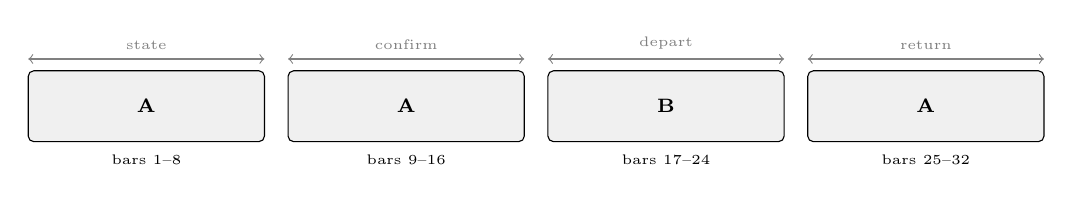
\begin{tikzpicture}[x=1cm,y=1cm,font=\scriptsize]
  \foreach \i/\lab/\x/\a/\b in {0/A/0/1/8,1/A/3.3/9/16,2/B/6.6/17/24,3/A/9.9/25/32} {
    \draw[rounded corners=2pt,fill=gray!12] (\x,0) rectangle ++(3.0,0.9);
    \node at (\x+1.5,0.45) {\textbf{\lab}};
    \node[below,font=\tiny] at (\x+1.5,-0.04) {bars \a--\b};
  }
  \draw[<->,gray] (0,1.05) -- (3.0,1.05) node[midway,above,font=\tiny]{state};
  \draw[<->,gray] (3.3,1.05) -- (6.3,1.05) node[midway,above,font=\tiny]{confirm};
  \draw[<->,gray] (6.6,1.05) -- (9.6,1.05) node[midway,above,font=\tiny]{depart};
  \draw[<->,gray] (9.9,1.05) -- (12.9,1.05) node[midway,above,font=\tiny]{return};
\end{tikzpicture}

Figure 8-1: a thirty-two-bar AABA map. The four eight-bar blocks state, confirm, depart, and return; B need not be a new key, but it must have a recognisable different direction.
\end{minipage}
\end{center}

AABA's strength is a small memory load and a clean return. The listener only needs to recognise one A and gets a familiar close at the end. B offers a controlled departure without dismantling the song. The risk is flatness: if all three A passes use the same lyric, arrangement, and rhythm, the last one feels like filler; if B only continues A's chords, there is no real departure.

To write AABA, first settle A's four-bar question and four-bar answer, then change the answer's final note or rhythm once to get A'. B can move to the relative minor, the subdominant, or simply change rhythmic density and register. The final A need not return literally; raise the last phrase, change the instrumentation, or add harmony so the return weighs more than the first statement.

\section{Common form two: verse--chorus}

Verse--chorus is the default form of modern pop, rock, and folk. It does not rely on one large section repeating; it alternates two functions. The verse carries narrative, setup, and lower energy. The chorus carries the title, the emotional high point, and the hook. A pre-chorus often climbs between them, and a bridge or instrumental can appear later.

A common eight-part skeleton is intro--verse 1--chorus 1--verse 2--chorus 2--bridge--chorus 3--outro. Each verse changes lyric; each chorus keeps the same core line; the bridge leaves the harmonic and rhythmic habits of both; the final chorus pushes the energy highest and a short outro lands it.

Verse and chorus differ by more than lyric position. Verses usually sit lower, use speech-like rhythm, and keep the arrangement thinner. Choruses sit higher, use opener vowels, fill the drums and low end, and land the title on a strong beat. The pre-chorus connects the two ends: it often shortens phrases, raises harmonic tension, adds a rising line, or accelerates the drums so the chorus has a launch.

\begin{center}
\small
\begin{tabular}{p{0.16\linewidth}p{0.24\linewidth}p{0.22\linewidth}p{0.20\linewidth}}
\toprule
Form & Strengths & Risks & Best for \\
\midrule
AABA & Small memory load, clean close, good for short pieces & Three A passes can flatten; B can become just ``different chords'' & Jazz standards, classic pop, short narratives \\
Verse--chorus & Clear emotional arc; the chorus can be reinforced & Verses can become waiting rooms; the bridge can be redundant & Modern pop, rock, folk, short-form songs \\
\bottomrule
\end{tabular}

Table 8-2: how AABA and verse--chorus divide the work. Neither form is superior; they put the weight in different places.
\end{center}

To write verse--chorus, fix the chorus title and its harmonic landing first, then write a verse that does not compete with it. If the verse already uses the chorus's register, density, and accents, the chorus has nowhere to rise. If the chorus is only a faster verse, it has no real gear change. A pre-chorus is optional, but when verse and chorus are far apart in register or rhythm, it is the cheapest bridge.


\begin{center}
\begin{minipage}{0.94\linewidth}
\centering
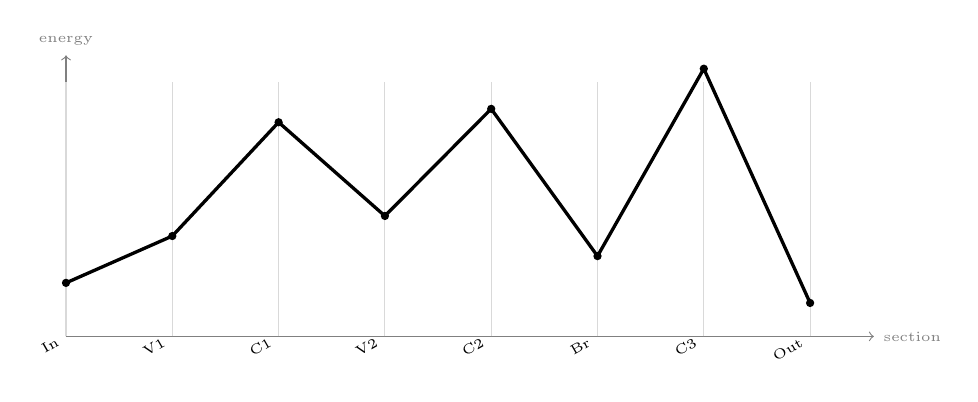
\begin{tikzpicture}[x=1.35cm,y=0.85cm,font=\scriptsize]
  \draw[->,gray] (0,0) -- (7.6,0) node[right,font=\tiny]{section};
  \draw[->,gray] (0,0) -- (0,4.2) node[above,font=\tiny]{energy};
  \foreach \x/\lab in {0/In,1/V1,2/C1,3/V2,4/C2,5/Br,6/C3,7/Out} {
    \draw[gray!30] (\x,0) -- (\x,3.8);
    \node[below,font=\tiny,rotate=30,anchor=east] at (\x,0) {\lab};
  }
  \draw[very thick] plot coordinates {(0,0.8) (1,1.5) (2,3.2) (3,1.8) (4,3.4) (5,1.2) (6,4.0) (7,0.5)};
  \foreach \x/\y in {0/0.8,1/1.5,2/3.2,3/1.8,4/3.4,5/1.2,6/4.0,7/0.5} {
    \fill (\x,\y) circle (1.5pt);
  }
\end{tikzpicture}

Figure 8-2: the energy curve of verse--chorus. The bridge deliberately dips, the final chorus rises highest, and the outro falls quickly; the curve shows relative energy, not exact pitch or volume.
\end{minipage}
\end{center}

\section{Transitions: giving the next section a reason to start}

The worst transition is a hard cut into what sounds like another song. A transition does not need to be long, but it needs an audible signal: a tempo change, harmonic tension, a drum fill, a register lift, a motive hand-off, or a clear rest. Four types cover most pop writing.

\begin{center}
\small
\begin{tabular}{p{0.20\linewidth}p{0.38\linewidth}p{0.30\linewidth}}
\toprule
Transition & How it works & Watch out for \\
\midrule
Hard cut & The previous section ends and the next starts directly on a strong beat & Good for a short, forceful chorus; too abrupt if key or register jumps far \\
Drum fill & Add snare, toms, or accelerating singles in the last one or two beats & The most general lift; too much fill steals the chorus downbeat \\
Riser / fall & Use a riser, reverse cymbal, noise, or string glide to push up or down & Align the rise with the chorus landing; too long becomes waiting \\
Common chord / motive & Pivot on a chord, motive, or melody note shared by both sections & Most natural and easiest to miss; plant it one beat early \\
\bottomrule
\end{tabular}

Table 8-3: four common section transitions. Decide which beat the next section starts on, then work backwards to the transition length.
\end{center}

A practical checklist: do the last two beats of the transition have a clear acceleration or pause? Does the next section's first accent land where the listener expects? Is the motive used in the transition picked up by the next section? If all three answers are no, the transition is probably just two sections cut together.

\section{How to do it in Yeban}

Yeban's arrangement view is good for laying out structure; it will not decide the structure for you. Write the sections and bar ranges on paper first, then place clips in the project.

\begin{enumerate}
  \item Write a structure table first: for example A bars 1--8, A' bars 9--16, B bars 17--24, A'' bars 25--32. Put each section's function (state, confirm, depart, return) beside it.
  \item Select a clip and press \texttt{Ctrl+C} to copy, \texttt{Ctrl+V} to paste. Paste lands on the selected track at the playhead, and multiple clips keep their relative spacing. \texttt{Ctrl+X} cuts.
  \item To repeat the selected clip immediately after itself, press \texttt{Ctrl+D}: with no note selection, it duplicates the selected arrangement clip, places the copy at the end of the original, and appends `` (Copy)'' to the clip name. If the piano roll still has a note selection, \texttt{Ctrl+D} duplicates the notes instead, not the whole clip.
  \item Use the track headers or mixer to confirm each track's role (drums, bass, chords, melody). Track and clip names are read-only in the current GUI: the track header and mixer have no rename field, and new clips get generated names such as \texttt{Clip} and \texttt{Clip 2}. To rename, use MCP \texttt{setTrackName} / \texttt{setClipName}; the GUI rename entry is not yet available.
  \item The section band above the arrangement shows existing \texttt{sections} (name, colour, start/end position); clicking a section card seeks the playhead to its start. The current GUI cannot create, drag, or rename sections on the band; section data must come from the project file or MCP \texttt{setSection}.
  \item Open the song overview and check that section boundaries line up with bar numbers. If the band is empty, the project has no \texttt{sections}; that is not a broken UI.
\end{enumerate}

\screenshot{arrangement-aaba-structure}{AABA section structure in the arrangement view}{AABA section structure in the arrangement view}

\textbf{Scope note:} Yeban currently has no automatic form analysis, section detection, section naming, or ``generate a whole song from a structure'' feature. The section band only reads existing \texttt{sections}; it does not infer them from audio or MIDI. Clip copy duplicates placement and clip references, not lyrics, arrangement, or chords. Structural judgment still comes from your ears and manual layout.

\section{Song form and energy steps in real songs}

\begin{itemize}
  \item \textbf{The Weeknd, ``Blinding Lights''}: Opens with the synth hook, strips back for the verse, climbs through the pre-chorus and blooms in the chorus—a textbook modern pop arc.
  \item \textbf{Adele, ``Rolling in the Deep''}: Starts with bare guitar and claps, then adds kick, piano, strings and backing vocals section by section so arrangement density marks form boundaries.
  \item \textbf{Zhao Lei, ``Chengdu'' (成都)}: Holds back to acoustic guitar and close vocal in the verse before strings and chorus voices lift the refrain.
\end{itemize}

\section{Exercises}


\begin{exercise}
\begin{enumerate}
  \item Write the bar ranges of a thirty-two-bar AABA and state B's function.
  \par\noindent Answer: A bars 1--8, A' bars 9--16, B bars 17--24, A'' bars 25--32. B departs from the main direction and provides contrast and a turn; the final A returns to close.
  \item Where would you put a pre-chorus between an eight-bar verse and an eight-bar chorus, and what must it accomplish?
  \par\noindent Answer: between the end of the verse and the start of the chorus, usually four to eight bars; it should shorten phrases, raise harmonic tension, or accelerate the drums to connect the verse's lower energy to the chorus's high point.
  \item What is the listening difference between repeating a four-bar phrase exactly four times and turning it into AABA?
  \par\noindent Answer: four exact passes only confirm and can flatten; AABA introduces B on the third pass, giving the ear a controlled departure before the return.
  \item Design a two-bar transition from verse to chorus: name the signal, the landing, and the risk.
  \par\noindent Answer: open-ended. A valid answer needs an audible signal (drum fill, riser, common chord, or motive bridge), a clear chorus downbeat, and a risk control (for example, the riser must not cover the chorus downbeat).
  \item In Yeban, copy the clip in bars 1--4 to bars 5--8, then copy it to another track. State the operation and its prerequisites.
  \par\noindent Answer: select the clip, \texttt{Ctrl+C}, select the target track, put the playhead at bar 5, \texttt{Ctrl+V}; to copy to another track, switch the selected track before pasting. To repeat it immediately after itself, \texttt{Ctrl+D} also works, but clear any note selection in the piano roll first.
\end{enumerate}
\end{exercise}

\section{Help topic map}

\begin{center}
\small
\begin{tabular}{p{0.26\linewidth}p{0.45\linewidth}p{0.18\linewidth}}
\toprule
Section & In-app help anchor & Note \\
\midrule
Form and levels & \texttt{music-theory-form} & concept \\
Repetition and variation & \texttt{music-theory-repetition-variation} & Table 8-1 \\
AABA & \texttt{music-theory-aaba} & Figure 8-1 \\
Verse--chorus & \texttt{music-theory-verse-chorus} & Table 8-2 \\
Transitions & \texttt{music-theory-transition} & Table 8-3 \\
How to in Yeban & \texttt{music-theory-arrangement-structure} & clips and section band \\
Exercises & \texttt{music-theory-ch8-practice} & answers at chapter end \\
\bottomrule
\end{tabular}
\end{center}

\section*{Further reading}
\begin{itemize}
  \item \textbf{Open Music Theory, “The small binary.”} \url{https://openmusictheory.github.io/smallBinary.html} — uses two-part form to show repetition, contrast, and return, the simplest structural skeleton.
  \item \textbf{YouTube, “The Hidden Structure Behind Every Song You’ve Ever Heard.”} \url{https://www.youtube.com/watch?v=v8fXuLi9Rb4} — a two-minute overview that links notes, rhythm, melody, harmony, and form.
\end{itemize}

